\documentclass[aspectratio=169]{beamer}


\mode<presentation>
{
  \usetheme{Antibes}

  \setbeamercovered{transparent}
}



\usepackage[french]{babel}
\usepackage[utf8]{inputenc}
\usepackage{times}
\usepackage[T1]{fontenc}
\usepackage{xcolor}
\usepackage{booktabs}
\usepackage{threeparttable}
\usepackage{tabularx}
\usepackage{caption}
\usepackage{numprint}
\usepackage{amsmath,amsfonts,amsthm,bm,nccmath}
\usepackage[export]{adjustbox}
\usepackage{tikz}
\usepackage{float}
\usepackage{listings}
\usepackage{textcomp}
\usepackage[backend=biber, style=authoryear, defernumbers=true]{biblatex}

\addbibresource{MyLibrary.bib}

\renewcommand*{\bibfont}{\scriptsize}

\captionsetup{font=scriptsize, labelfont=scriptsize}

\date{8 décembre 2022}

%\usefonttheme[onlymath]{serif}

\definecolor{my_blue}{rgb}{0.3, 0.4, 0.5}
\definecolor{my_grey}{rgb}{0.6, 0.6, 0.6}

\usecolortheme[named = my_blue]{structure}

\setbeamertemplate{footline}{}

\setbeamerfont{author in head/foot}{size=\fontsize{4}{4.8}\selectfont}

\setbeamertemplate{bibliography item}{}
\setbeamertemplate{bibliography entry article}{}
\setbeamertemplate{bibliography entry title}{}
\setbeamertemplate{bibliography entry location}{}
\setbeamertemplate{bibliography entry note}{}


\setbeamerfont{bibliography entry author}{size=\footnotesize}
\setbeamerfont{bibliography entry title}{size=\footnotesize}
\setbeamerfont{bibliography entry location}{size=\footnotesize}
\setbeamerfont{bibliography entry note}{size=\footnotesize}

\defbeamertemplate{footline}{myframe number}
{
  \hfill%
  \usebeamercolor[fg]{page number in head/foot}%
  \usebeamerfont{page number in head/foot}%
  \raisebox{0.3cm}[0pt][0pt]{% <--- change here
    \insertframenumber\,/\,\inserttotalframenumber\kern1em}%
}

\setbeamertemplate{footline}[myframe number]
\beamertemplatenavigationsymbolsempty

\newcommand\Wider[2][3em]{%
\makebox[\linewidth][c]{%
  \begin{minipage}{\dimexpr\textwidth+#1\relax}
  \raggedright#2
  \end{minipage}%
  }%
}


\title{Modélisation nonstationnaires des valeurs extrêmes par reversible jump Markov chain Monte Carlo}

\author{Antoine~Chapon~et Jean Truchard Saint Clore}

\institute[Universities of Somewhere and Elsewhere] % (optional, but mostly needed)
{
  cours ETE 405
 }
% - Use the \inst command only if there are several affiliations.
% - Keep it simple, no one is interested in your street address.

%\date[CFP 2003] % (optional, should be abbreviation of conference name)
%{Conference on Fabulous Presentations, 2003}
% - Either use conference name or its abbreviation.
% - Not really informative to the audience, more for people (including
%   yourself) who are reading the slides online

%\subject{Theoretical Computer Science}
% This is only inserted into the PDF information catalog. Can be left
% out. 



% If you have a file called "university-logo-filename.xxx", where xxx
% is a graphic format that can be processed by latex or pdflatex,
% resp., then you can add a logo as follows:

% \pgfdeclareimage[height=0.5cm]{university-logo}{university-logo-filename}
% \logo{\pgfuseimage{university-logo}}



% Delete this, if you do not want the table of contents to pop up at
% the beginning of each subsection:
\AtBeginSubsection[]
{
\begin{frame}<beamer>{Plan}
\frametitle{Plan}
\tableofcontents[currentsection,currentsubsection]
\end{frame}
}


% If you wish to uncover everything in a step-wise fashion, uncomment
% the following command: 

%\beamerdefaultoverlayspecification{<+->}


\begin{document}

\begin{frame}
  \titlepage
\end{frame}



\section*{}

%\begin{frame}{Introduction}
%	\begin{itemize}
%	\setlength{\itemsep}{10pt}
%	\item Occupation du sol (\emph{land use} -- LU).
%	\item Changement de LU $\rightarrow$ potentielle imperméabilisation.
%	\item Processus anthropique mais conditionné par des paramètres physiques.
%	\item La pente est un paramètre important.
%	\end{itemize}
%\vspace{0.5cm}
%Changement de LU dans 2 bassins versants (BV) d\rq{}Austin, en lien avec le relief.\\
%\vspace{0.5cm}
%		{\scriptsize
%		\cite{united_states_environmental_protection_agency_land_2017, exum_estimating_2005, fu_temporal_2006}}
%\end{frame}

\begin{frame}{Plan}
\tableofcontents
\end{frame}


\section{Modèle des valeurs extrêmes par dépassement de seuil}

\begin{frame}{Seuil par régression quantile}
\begin{columns}
	\begin{column}{0.4\textwidth}
		\begin{figure}
		\vspace{-0.4cm}
	 		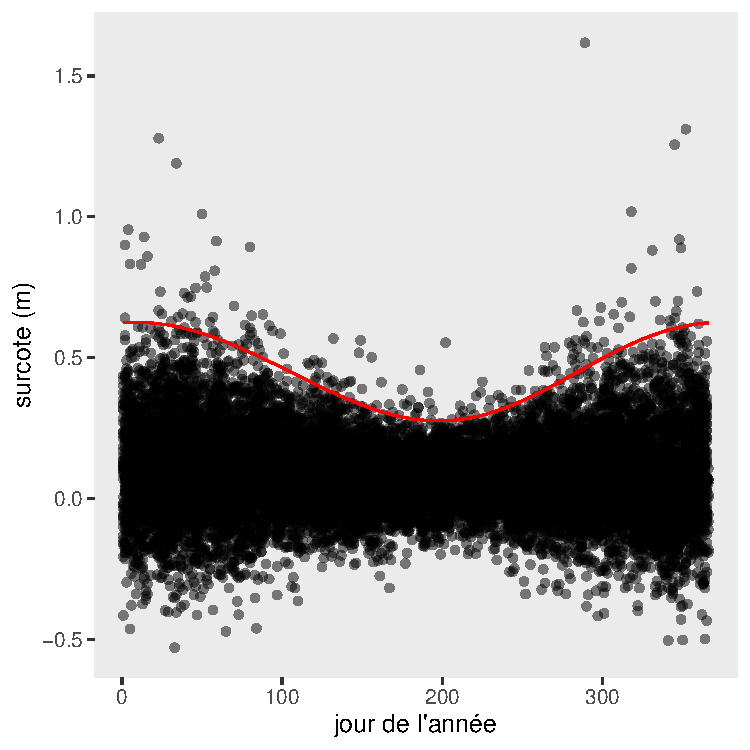
\includegraphics[height=0.85\textheight, center]{../figures/points.pdf}
		\end{figure}
	\end{column}
	\begin{column}{0.6\textwidth}
	Régression quantile en fonction de la saison avec une probabilité journalière de dépassement de 1 \%.
	\end{column}
\end{columns}
\end{frame}

\begin{frame}{Nonhomogeneous Poisson process}
\begin{columns}
	\begin{column}{0.5\textwidth}
		Intensité du point process définie par
		\vspace{0.1cm} \\
		\begin{equation*}
		\lambda_b(t,y_t) = b^{-1}\sigma_t^{-1} \left( 1+\xi_t\dfrac{y_t-\mu_t}{\sigma_t} \right)^{-1/\xi_t-1}
		\end{equation*}
		\vspace{0.2cm} \\
		avec $1+\xi_t(y_t-\mu_t)/\sigma_t > 0$, \\ sinon $\lambda_b(t,y_t) = 0$.
	\end{column}
	\begin{column}{0.5\textwidth}
	\vspace{0.5cm} \\
		Paramètres dépendants de $t$ et $s_t$ avec comme modèle ayant le plus d'hyperparamètres
		\begin{fleqn}
		\begin{equation*}
		\mu_t = \mu_0 + \mu_1 t + \mu_2 t^2 + \mu_3 \cos(s_t) + \mu_4 \sin(s_t),
		\end{equation*}
		\begin{equation*}
		\phi_t = \phi_0 + \phi_1 t + \phi_2 t^2 + \phi_3 \cos(s_t) + \phi_4 \sin(s_t),
		\end{equation*}
		\begin{equation*}
		\sigma_t = \exp(\phi_t),
		\end{equation*}
		pour que $\sigma_t > 0$ et
		\begin{equation*}
		\xi_t = \xi.
		\end{equation*}
		\end{fleqn}
	\end{column}
\end{columns}
	\vspace{1cm}
	{\scriptsize
	\cite{northrop_threshold_2016}}
\end{frame}



\begin{frame}{Sauts entre les modèles}
	\begin{figure}
	\vspace{-0.15cm}
	 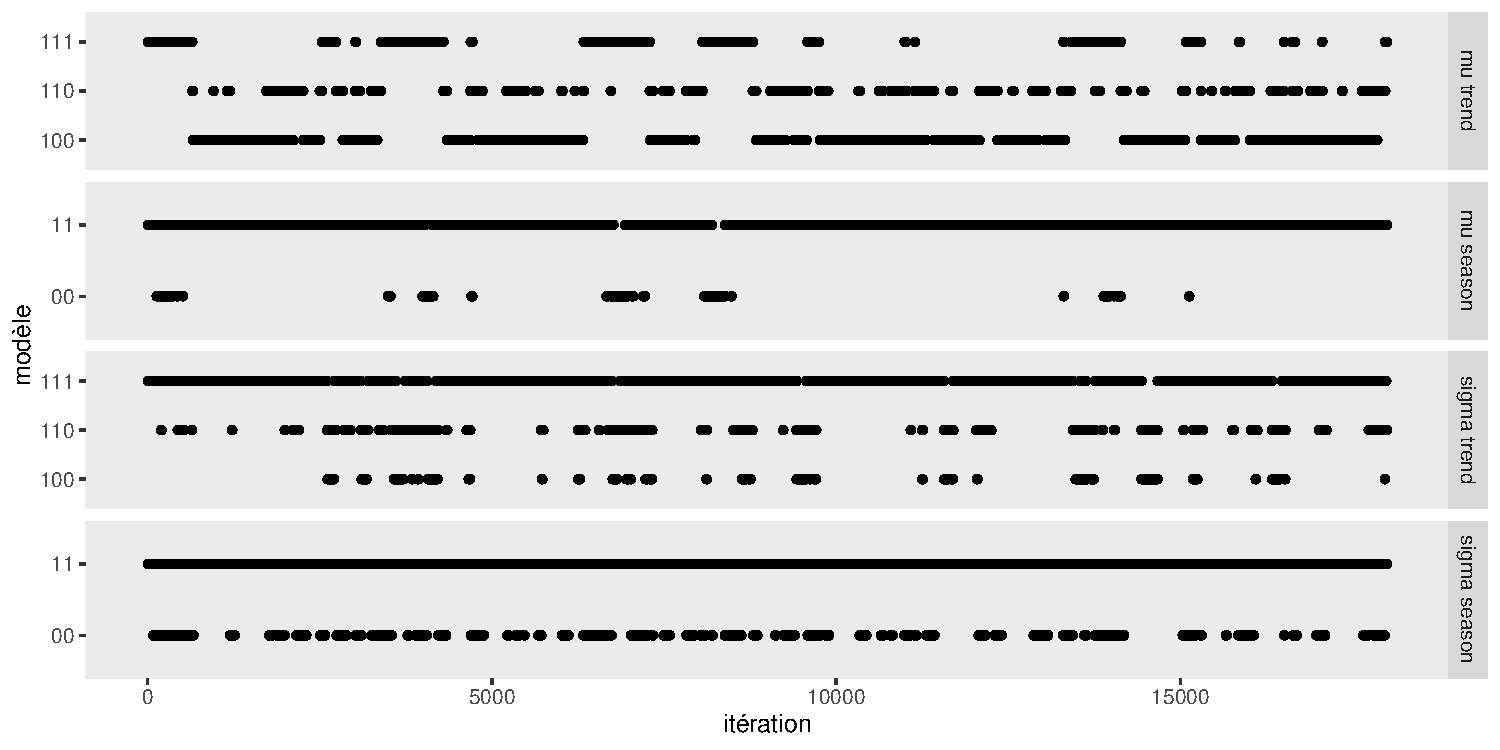
\includegraphics[width=0.95\textwidth, center]{../figures/jumps.pdf}
	\end{figure}
\end{frame}


\begin{frame}{Modèles visités}
\begin{columns}
	\begin{column}{0.4\textwidth}
		\begin{figure}
		\vspace{-0.4cm}
	 		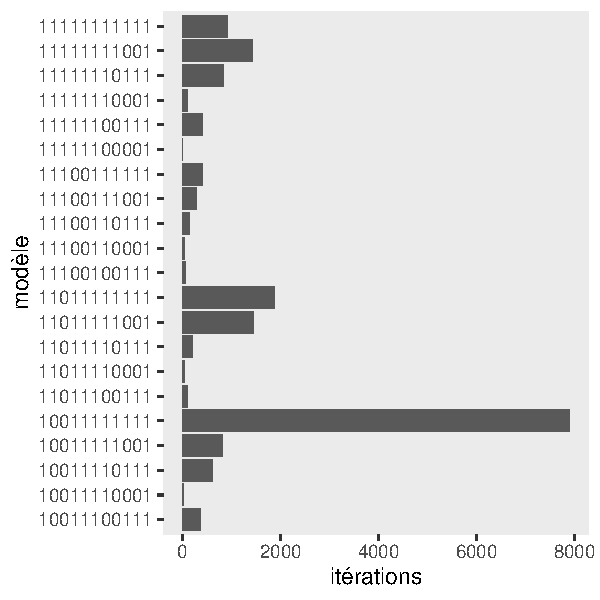
\includegraphics[height=0.85\textheight, center]{../figures/models.pdf}
		\end{figure}
	\end{column}
	\begin{column}{0.6\textwidth}
    Le modèle paramétrisé
    \begin{fleqn}
    \begin{equation*}
		\mu_t = \mu_0 + \mu_3 \cos(s_t) + \mu_4 \sin(s_t),
	\end{equation*}
	\begin{equation*}
		\sigma_t = \exp(\phi_0 + \phi_1 t + \phi_2 t^2 + \phi_3 \cos(s_t) + \phi_4 \sin(s_t)),
	\end{equation*}
	\begin{equation*}
		\xi_t = \xi,
	\end{equation*}
	\end{fleqn}
	est le plus visité.
	\end{column}
\end{columns}
\end{frame}


\begin{frame}{Graphiques de trace}
\begin{columns}
	\begin{column}{0.7\textwidth}
		\begin{figure}
		\vspace{-0.4cm}
	 		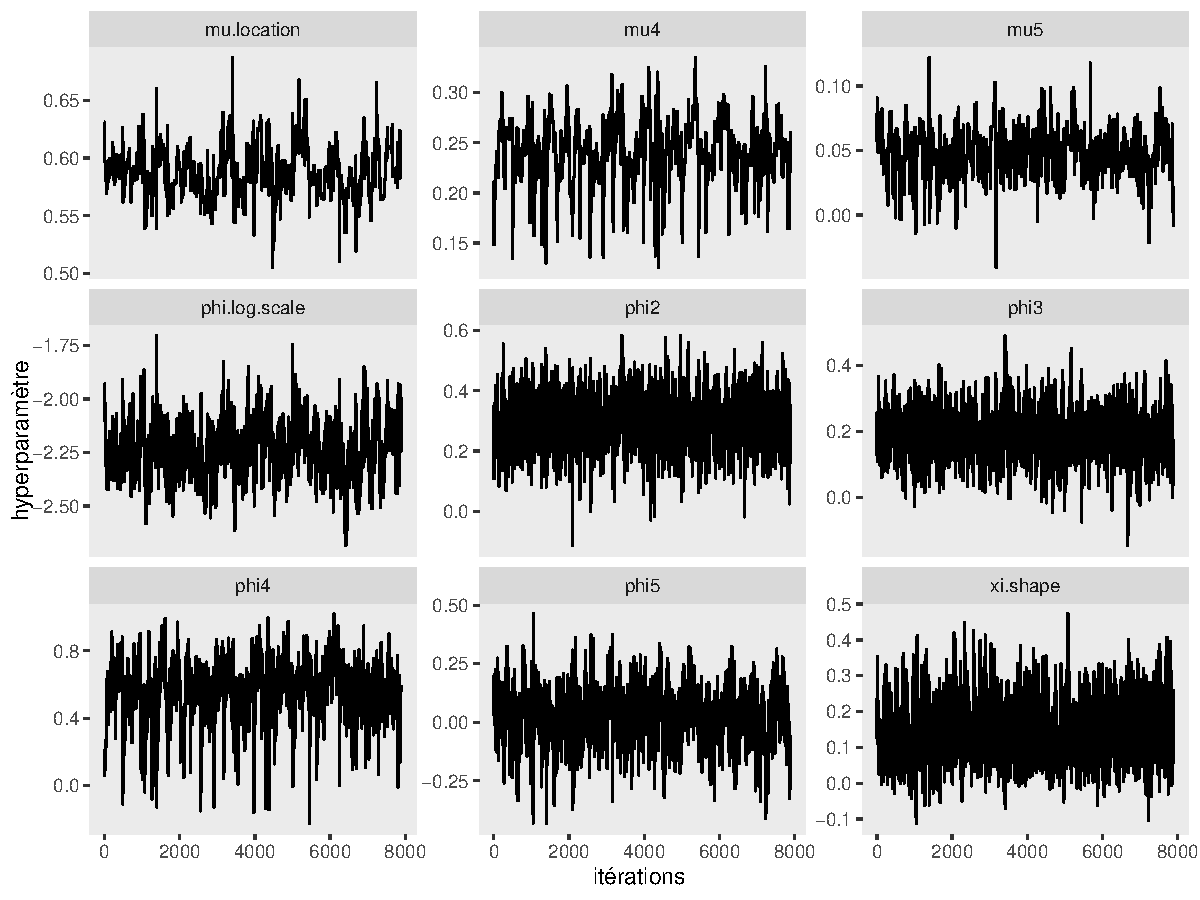
\includegraphics[height=0.85\textheight, center]{../figures/traces.pdf}
		\end{figure}
	\end{column}
	\begin{column}{0.3\textwidth}
    Pseudo traces pour les 9 hyperparamètres du modèle le plus visité.
	\end{column}
\end{columns}
\end{frame}


\begin{frame}{Distributions des hyperparamètres}
\begin{columns}
	\begin{column}{0.7\textwidth}
		\begin{figure}
		\vspace{-0.4cm}
	 		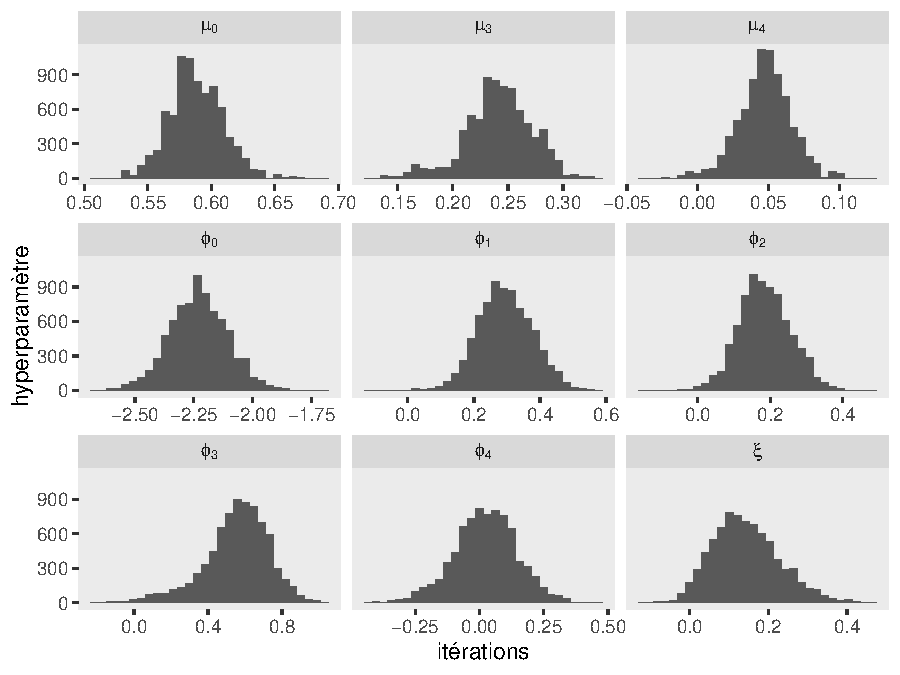
\includegraphics[height=0.85\textheight, center]{../figures/hists.pdf}
		\end{figure}
	\end{column}
	\begin{column}{0.3\textwidth}
	Hyperparamètres du modèle le plus visité.
	\end{column}
\end{columns}
\end{frame}


%\section{Site d\rq{}étude et données}
%
%\subsection{Localisation des bassins versants dans l\rq{}aire urbaine d\rq{}Austin}
%
%\begin{frame}
%\begin{columns}
%	\begin{column}{0.75\textwidth}
%		\begin{figure}
%	 		\includegraphics[height=0.95\textheight, center]{intro_map.png}
%		\end{figure}
%	\end{column}
%	\begin{column}{0.25\textwidth}
%             	Zoom avec \emph{overview}.\\
%		\vspace{1cm}
%		{\scriptsize
%		\cite{united_states_census_bureau_census_2020, united_states_census_bureau_us_2021}}
%	\end{column}
%\end{columns}
%\end{frame}
%
%\subsection{Données d\rq{}occupation des sols}
%
%\begin{frame}
%\begin{columns}
%	\begin{column}{0.5\textwidth}
%		\begin{itemize}
%		\setlength{\itemsep}{10pt}
%		\item LU fournies pour 1990, 1995, 2000 et 2003.
%		\item Autres données disponibles pour 2010 et une date non-spécifiée.
%		\item Polygones avec classe de LU.
%		\item Données partiellement ou totalement inutilisables.
%		\end{itemize}
%	\end{column}
%	\begin{column}{0.5\textwidth}
%		\begin{itemize}
%		\setlength{\itemsep}{10pt}
%		\item Extraction des parcelles dans les BVs.
%		\item Recalcul de l\rq{}aire des parcelles.
%		\item Jointure de toutes les données de LU aux parcelles de 2010.
%		\item Polygones des routes absents en 2010 : calcul de la différence avec le  BV et fusion avec les autres parcelles.
%		\end{itemize}
%	\end{column}
%\end{columns}
%	\vspace{1cm}
%	{\scriptsize
%	\cite{city_of_austin_planning_and_development_review_2010_2021, city_of_austin_planning_and_development_review_land_2021}}
%\end{frame}
%
%\subsection{Données de topographie}
%
%\begin{frame}
%	\begin{figure}
%	 	\includegraphics[width=1.1\textwidth, center]{MNT_correction.png}
%	\end{figure}
%Décalage estimé par outils de mesure, puis correction des coordonnées ($‐50$ m en X et $+200$ m en Y).
%\end{frame}
%
%
%\section{Occupation des sols et urbanisation}
%
%\subsection{Méthode d\rq{}analyse de l\rq{}évolution de l\rq{}urbanisation}
%
%\begin{frame}{Classes d\rq{}occupation des sols}
%\begin{table}[ht]
%\centering
%\scriptsize
%\begin{tabularx}{\textwidth}{lllll}
%  \toprule
%indice urbanisation & classe simple & nom classe & classe complète & définition \\ 
%  \midrule
%  0 &   7 & espace verts & 700 & ? \\ 
%     &    &  & 710 & Parks/Greenbelts  \\ 
%     &    &  & 720 & Golf Courses  \\ 
%\vdots &  \vdots & \vdots & \vdots & \vdots \\
%     &   9 & agricole ou naturel & 910 & Agricultural \\ 
%     &    &  & 940 & Water  \\ 
%     &    &  & 999 & Unknown \\ 
%     \midrule
%\vdots &  \vdots & \vdots & \vdots & \vdots \\
%     \midrule
%    3 &   5 & industrie & 500 & ? \\ 
%\vdots &  \vdots & \vdots & \vdots & \vdots \\
%     &   8 & route ou transport & 800 & ? \\ 
%\vdots &  \vdots & \vdots & \vdots & \vdots \\
%   \bottomrule
%\end{tabularx}
%\end{table}
%\end{frame}
%
%\begin{frame}{Indice d\rq{}urbanisation}
%\begin{columns}
%	\begin{column}{0.5\textwidth}
%	\begin{block}{Calcul de champ}
%	CASE\\
%	WHEN LU1990 in (7, 9) THEN 0\\
%	WHEN LU1990 in (0, 1, 3) THEN 1\\
%	WHEN LU1990 in (2, 4, 6) THEN 2\\
%	WHEN LU1990 in (5, 8) THEN 3\\
%	END
%	\end{block}
%	\end{column}
%	\begin{column}{0.5\textwidth}
%		\begin{itemize}
%		\setlength{\itemsep}{10pt}
%		\item \lq\lq{}potentiel de ruissellement\rq\rq{} de la classe de LU.
%		\item Indice ordonné.
%		\item Permet de calculer une évolution.
%		\end{itemize}
%	\end{column}
%\end{columns}
%\end{frame}
%
%\subsection{Évolution de l\rq{}occupation des sols de 1990 à 2010}
%
%\begin{frame}
%\begin{columns}
%	\begin{column}{0.75\textwidth}
%	\begin{figure}
%	 	\includegraphics[height=0.97\textheight, center]{LandUse_Bull.png}
%	\end{figure}
%	\end{column}
%	\begin{column}{0.25\textwidth}
%	\begin{figure}
%	 	\begin{itemize}
%		\item Résultats présentés uniquement pour le BV de Bull.
%		\item Pas de routes en 1990 ?
%		\item Encore plus de problèmes pour le BV de Williamson.
%		\end{itemize}
%	\end{figure}
%	\end{column}
%\end{columns}
%\end{frame}
%
%\begin{frame}{Évolution de l\rq{}occupation pour le BV de Bull}
%\begin{columns}
%	\begin{column}{0.77\textwidth}
%		 \includegraphics[height=0.8\textheight, center]{LUbull_area.pdf}
%	\end{column}
%	\begin{column}{0.23\textwidth}
%		 \begin{itemize}
%		\item Diminution classe 9.
%		\item Augmentation classes 7 et 1.
%		\item Stabilité classe 8.
%		\item Disparition de la classe 0 en 2003, impact ?
%		\end{itemize}
%	\end{column}
%\end{columns}
%\end{frame}
%
%\begin{frame}{Évolution de l\rq{}indice d\rq{}urbanisation pour le BV de Bull}
%\includegraphics[width=1.13\textwidth ,center]{DeltaUrb.png}
%\end{frame}
%
%
%\section{Relation entre topographie, pente et occupation des sols}
%
%\subsection{Méthodes d\rq{}analyse des données topographiques}
%
%\begin{frame}{Création d\rq{}une couche avec LU, élévation et pente}
%	\begin{enumerate}
%	\setlength{\itemsep}{10pt}
%	\item Raster de pente créé à partir du MNT avec la fonction \emph{slope}.
%	\item Rasters de MNT et pente convertis en points.
%	\item Extraction des données de LU avec les points de MNT.
%	\item Jointure des points de LU, MNT et pente.
%	\item Couche exportable pour analyse dans R.
%	\end{enumerate}
%\end{frame}
%
%\subsection{Impact de la topographie sur l\rq{}occupation des sols et l\rq{}urbanisation}
%
%\begin{frame}{Topographie et pente du BV de Bull}
%\includegraphics[width=\textwidth, center]{topo_Bull.png}
%\end{frame}
%
%\begin{frame}{Lien \emph{local} entre relief et LU}
%\includegraphics[width=0.93\textwidth, center]{habitat_MNT.png}
%\end{frame}
%
%\begin{frame}{Topographie et pente du BV de Williamson et courbe hypsométrique}
%\begin{columns}
%	\begin{column}{0.65\textwidth}
%	\includegraphics[height=0.87\textheight, center]{topo_Williamson.png}
%	\end{column}
%	\begin{column}{0.35\textwidth}
%	\includegraphics[height=0.5\textheight, center]{courbe_hypso.pdf}
%	\end{column}
%\end{columns}
%\end{frame}
%
%\begin{frame}{Lien entre élévation et LU}
%\includegraphics[width=0.95\textwidth, center]{boxplot_MNT.pdf}
%\end{frame}
%
%\begin{frame}{Lien entre pente et LU}
%\includegraphics[width=0.95\textwidth, center]{boxplot_slope.pdf}
%\end{frame}
%
%\begin{frame}{Lien entre relief et la classe 5 \lq\lq{}industrie\rq\rq{}}
%\includegraphics[width=1.13\textwidth, center]{indus_slope.png}
%\end{frame}
%
%
%\section{Conclusion}
%
%\begin{frame}<beamer>{Plan}
%\frametitle{Plan}
%\tableofcontents[currentsection]
%\end{frame}
%
%\begin{frame}
% 	\begin{itemize}
% 	\setlength{\itemsep}{10pt}
%	\item Augmentation du degré d\rq{}urbanisation des BVs ...
%	\item ... principalement le long des routes majeures.
%	\item Pas de lien entre LU et altitude.
%	\item Quelques relations entre LU et pente.
%	\item Le réseau de transport semble plus déterminant que le relief ...
%	\item ... mais ce réseau pourrait aussi être dépendant du relief.
%	\item Plus de données devraient être analysées pour réellement conclure.
%	\end{itemize}
%\end{frame}

\section*{}

\begin{frame}[plain]{Références}
\printbibliography
\end{frame}

{
\setbeamercolor{background canvas}{bg=my_blue}
\begin{frame}[plain]
\begin{tikzpicture}[overlay, remember picture]
\node[anchor=center] at (current page.center) {
\begin{beamercolorbox}[center]{title}
     \centerline{\huge{\textcolor{white}{merci pour votre attention}}}
  \end{beamercolorbox}};
\end{tikzpicture}
\end{frame}
}


\end{document}


